\documentclass[14pt]{article}

% Basic packages
\usepackage{subfiles}
\usepackage{extsizes}
\usepackage[quiet]{fontspec}
\usepackage{unicode-math}
\usepackage[margin=2cm]{geometry}
\usepackage{hyperref}
\usepackage{fancyhdr, lastpage}
\usepackage{multirow, multicol}
\usepackage{longtable}
\usepackage{siunitx}
\usepackage{amsmath, amssymb}
\usepackage{soul}
\usepackage{float}
\usepackage{graphicx}
\usepackage{subcaption}
\usepackage{pdfpages}
\usepackage{changepage}

% Font config
\defaultfontfeatures{Scale=MatchUppercase}
\setmainfont{Libertinus Serif}
\setsansfont{Carlito}
\setmonofont{DejaVu Sans Mono}
\setmathfont{Libertinus Math}
\setul{1pt}{.4pt}

% Page layout config
\let\OLDTITLE\title
\renewcommand{\title}[1]{\OLDTITLE{#1}\newcommand{\thetitle}{#1}}
\pagestyle{fancy}
\lhead{\thetitle}
\cfoot{Page \thepage\ of \pageref{LastPage}}

% Hyperref config
\hypersetup{colorlinks=true, urlcolor=blue}
\urlstyle{same}

% Minted config
\usepackage[outputdir={\detokenize{OUTDIR}}]{minted}
\renewcommand{\theFancyVerbLine}{\sffamily
\textcolor[rgb]{0.4,0.4,0.4}{\small \arabic{FancyVerbLine}}}
\setminted{linenos,autogobble,obeytabs,frame=single,highlightcolor=yellow}
\renewcommand{\listingscaption}{Source}

% \usepackage[singlefile, pdf]{graphviz}

\title{Evolutionary Computation Lab I}
\author{Piotr Kaszubski 148283}
\date{Sunday, October 15, 2023}

\begin{document}
\maketitle
\tableofcontents
\newpage

\section{Problem description}
We are given three columns of integers with a row for each node. The first two
columns contain \verb`x` and \verb`y` coordinates of the node positions in a
plane. The third column contains node costs.

\begin{enumerate}
	\item Select exactly 50\% of the nodes (if the number of nodes is odd we
		round the number of nodes to be selected up).
	\item Form a Hamiltonian cycle (closed path) through this set of nodes such
		that the sum of the total length of the path plus the total cost of the
		selected nodes is minimized. The distances between nodes are calculated
		as Euclidean distances rounded mathematically to integer values.
\end{enumerate}

The distance matrix should be calculated just after reading an instance and
then only the distance matrix (no nodes coordinates) should be accessed by
optimization methods to allow instances defined only by distance matrices.

\section{Pseudocode}
\subsection{Random solution}
\begin{description}
	\item [Input] A set \verb`N` of nodes.
	\item [Output] An ordered subset \verb`N'` of \verb`N`, with half of
		\verb`N`'s cardinality.
	\item [Steps]
		\begin{enumerate}\item []
			\item Initialize \verb`N'` to an empty list.
			\item While \verb`[ len(N') < len(N)/2 ]`, do:
				\begin{enumerate}
					\item Choose a random node \verb`n` from \verb`N`.
					\item Remove \verb`n` from \verb`N`.
					\item Append \verb`n` to \verb`N'`.
				\end{enumerate}
		\end{enumerate}
\end{description}

\subsection{Nearest neighbor}
\begin{description}
	\item [Input] A set \verb`N` of nodes.
	\item [Output] An ordered subset \verb`N'` of \verb`N`, with half of
		\verb`N`'s cardinality.
	\item [Steps]
		\begin{enumerate}\item []
			\item Initialize \verb`N'` to an empty list.
			\item Choose a random node \verb`prev_n` from \verb`N`.
			\item Remove \verb`prev_n` from \verb`N`.
			\item Append \verb`prev_n` to \verb`N'`.
			\item While \verb`[ len(N') < len(N)/2 ]`, do:
				\begin{enumerate}
					\item Find the node \verb`n` from \verb`N` with the
						smallest distance to \verb`prev_n`.
					\item Set \verb`prev_n` to \verb`n`.
					\item Remove \verb`n` from \verb`N`.
					\item Append \verb`n` to \verb`N'`.
				\end{enumerate}
		\end{enumerate}
\end{description}

\subsection{Greedy cycle}
\begin{description}
	\item [Input] A set \verb`N` of nodes.
	\item [Output] An ordered subset \verb`N'` of \verb`N`, with half of
		\verb`N`'s cardinality.
	\item [Steps]
		\begin{enumerate}\item []
			\item Initialize \verb`N'` to an empty list.
			\item Choose a random node \verb`n1` from \verb`N`.
			\item Remove \verb`n1` from \verb`N`.
			\item Append \verb`n1` to \verb`N'`.
			\item Find the node \verb`n2` from \verb`N` with the smallest
				distance to \verb`n1`.
			\item Remove \verb`n2` from \verb`N`.
			\item Append \verb`n2` to \verb`N'`.
			\item While \verb`[ len(N') < len(N)/2 ]`, do:
				\begin{enumerate}
					\item Let \verb`found_n` be an empty value.
					\item Let \verb`lowest_delta` be infinity.
					\item For each pair \verb`(n,o)` of adjacent nodes from \verb`N'`, do:
						\begin{enumerate}
							\item Find the node \verb`p` from \verb`N`, such
								that the sum \verb`s` of its distances from
								\verb`n` and \verb`o` is minimal.
							\item Let \verb`delta` be \verb`s` minus the
								distance between \verb`n` and \verb`o`.
							\item If \verb`delta < lowest_delta`, then:
								\begin{enumerate}
									\item Set \verb`found_n` to \verb`p`.
									\item Set \verb`lowest_delta` to \verb`delta`.
								\end{enumerate}
						\end{enumerate}
					\item Remove \verb`found_n` from \verb`N`.
					\item Append \verb`found_n` to \verb`N'`.
				\end{enumerate}
		\end{enumerate}
\end{description}

\section{Results}
\begin{longtable}[c]{|cc|rrr|}
	\hline
	\textbf{ALG.} & \textbf{FILE} & \textbf{min} & \textbf{avg} & \textbf{max} \\
	\hline
	\endfirsthead
	\hline
	\textbf{ALG.} & \textbf{FILE} & \textbf{min} & \textbf{avg} & \textbf{max} \\
	\hline
	\endhead
	\multirow{3}*{random} & \verb`TSPA.csv` & 241,510 & 266,062 & 308,034 \\
	& \verb`TSPB.csv` & 241,731 & 266,549 & 293,093 \\
	& \verb`TSPC.csv` & 189,473 & 215,587 & 239,581 \\
	\hline

	\multirow{3}*{nn} & \verb`TSPA.csv` & 110,035 & 116,145 & 125,805 \\
	& \verb`TSPB.csv` & 106,815 & 116,181 & 124,675 \\
	& \verb`TSPC.csv` & 62,629 & 66,196 & 71,616 \\
	\hline

	\multirow{3}*{cycle} & \verb`TSPA.csv` & 113,298 & 123,691 & 129,175 \\
	& \verb`TSPB.csv` & 111,981 & 120,922 & 131,174 \\
	& \verb`TSPC.csv` & 67,077 & 72,771	 & 75,763 \\
	\hline
\end{longtable}

\section{Visualizations}

\subsection{TSPA.csv}
\begin{figure}[H]
	\begin{adjustwidth}{-3em}{0}
		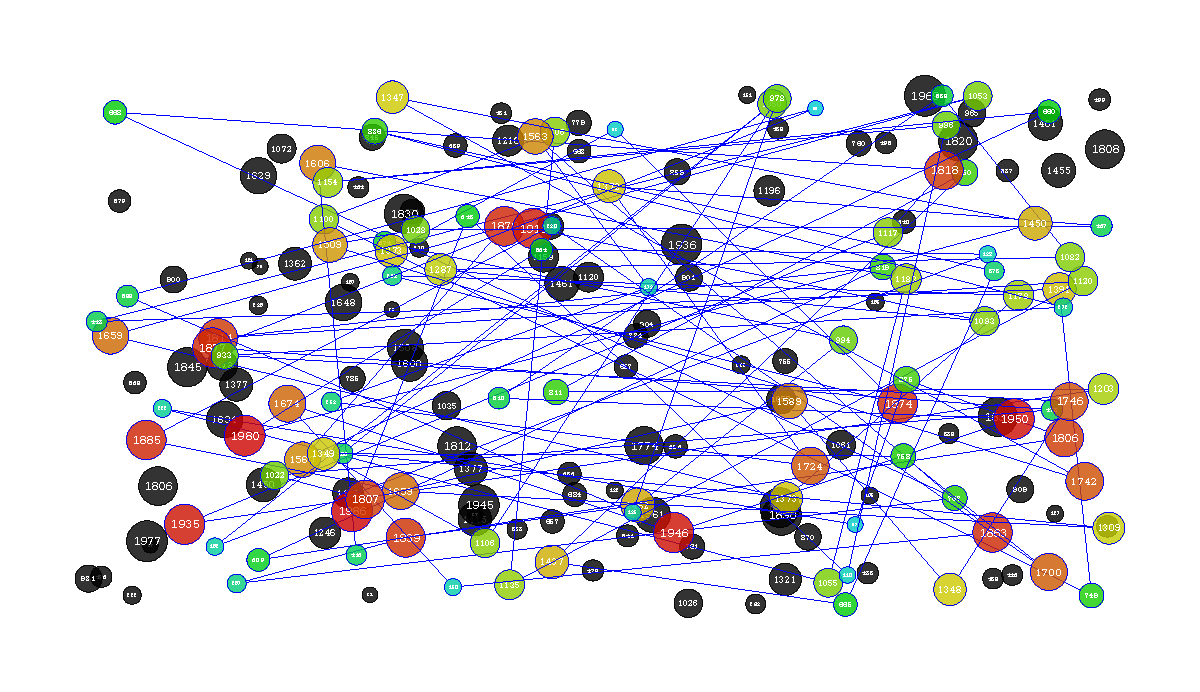
\includegraphics{results/best_random_TSPA.pdf}
	\end{adjustwidth}
	\vspace{-15mm}
	\caption{Best random solution to TSPA (241,510)}
\end{figure}
\begin{figure}[H]
	\begin{adjustwidth}{-3em}{0}
		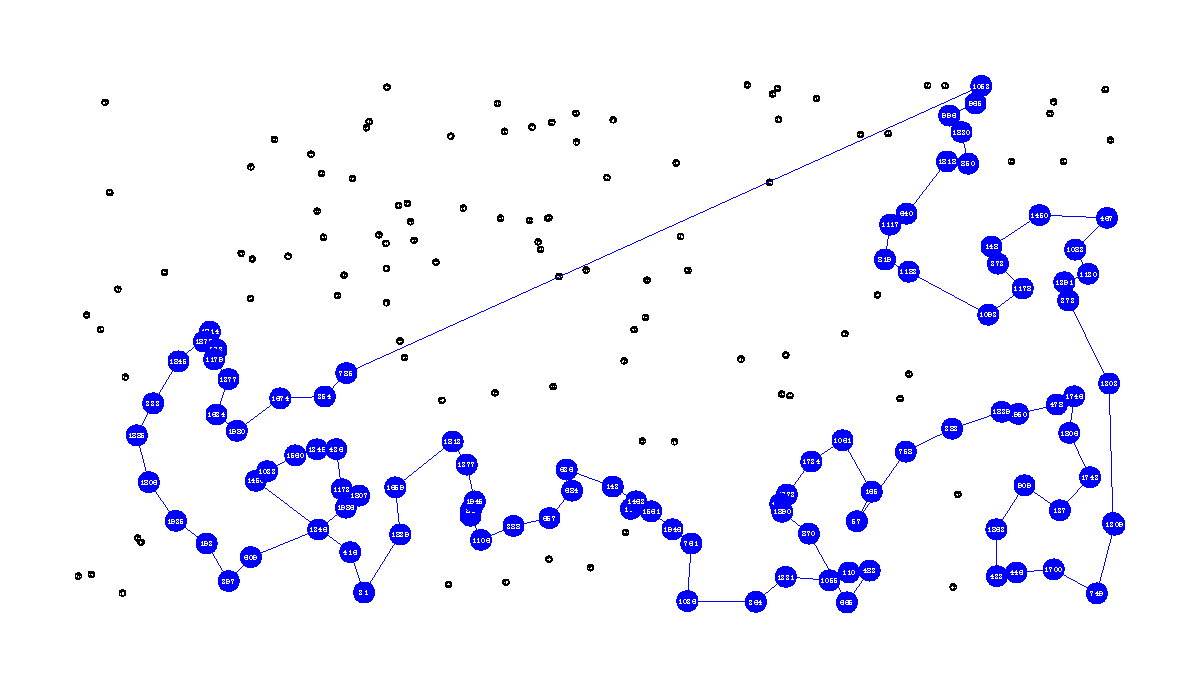
\includegraphics{results/best_nearest-neighbor_TSPA.pdf}
	\end{adjustwidth}
	\vspace{-15mm}
	\caption{Best nearest neighbor solution to TSPA (110,035)}
\end{figure}
\begin{figure}[H]
	\begin{adjustwidth}{-3em}{0}
		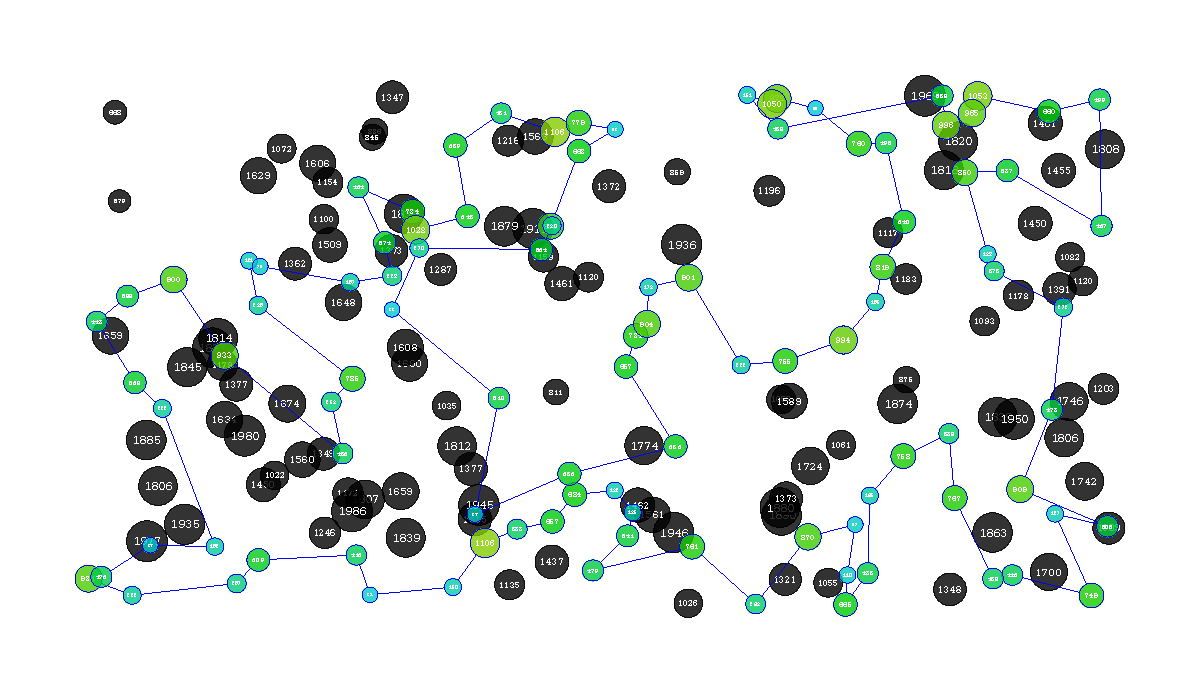
\includegraphics{results/best_greedy-cycle_TSPA.pdf}
	\end{adjustwidth}
	\vspace{-15mm}
	\caption{Best greedy cycle solution to TSPA (113,298)}
\end{figure}

\subsection{TSPB.csv}
\begin{figure}[H]
	\begin{adjustwidth}{-3em}{0}
		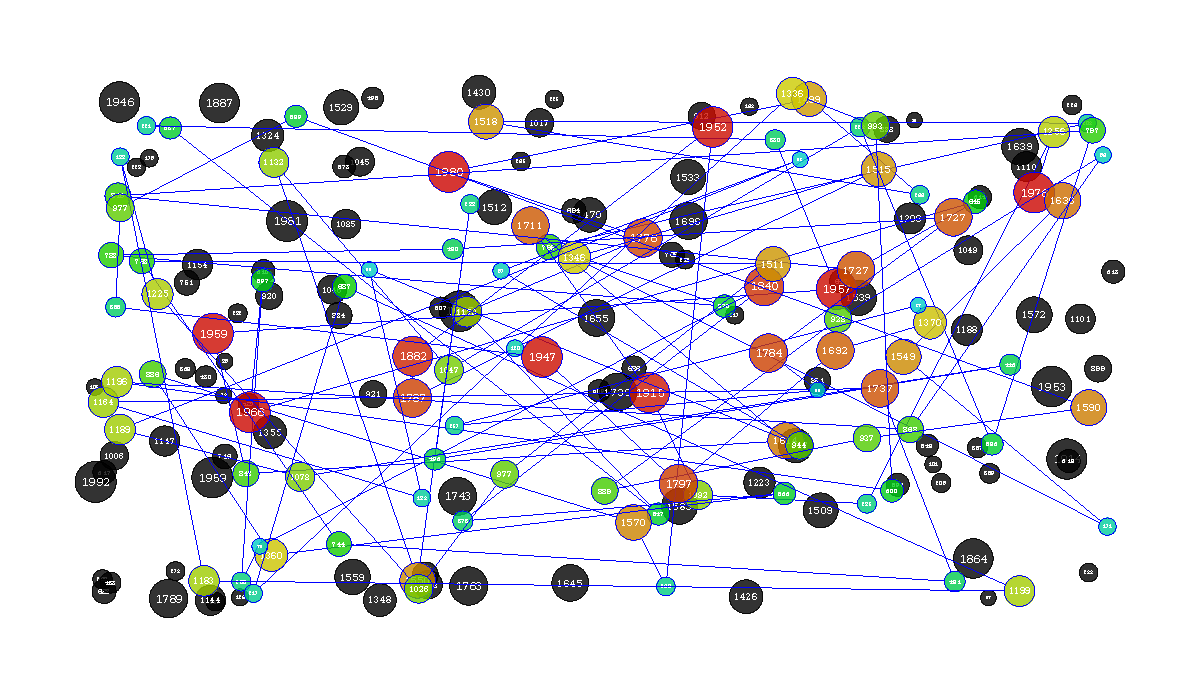
\includegraphics{results/best_random_TSPB.pdf}
	\end{adjustwidth}
	\vspace{-15mm}
	\caption{Best random solution to TSPB (241,731)}
\end{figure}
\begin{figure}[H]
	\begin{adjustwidth}{-3em}{0}
		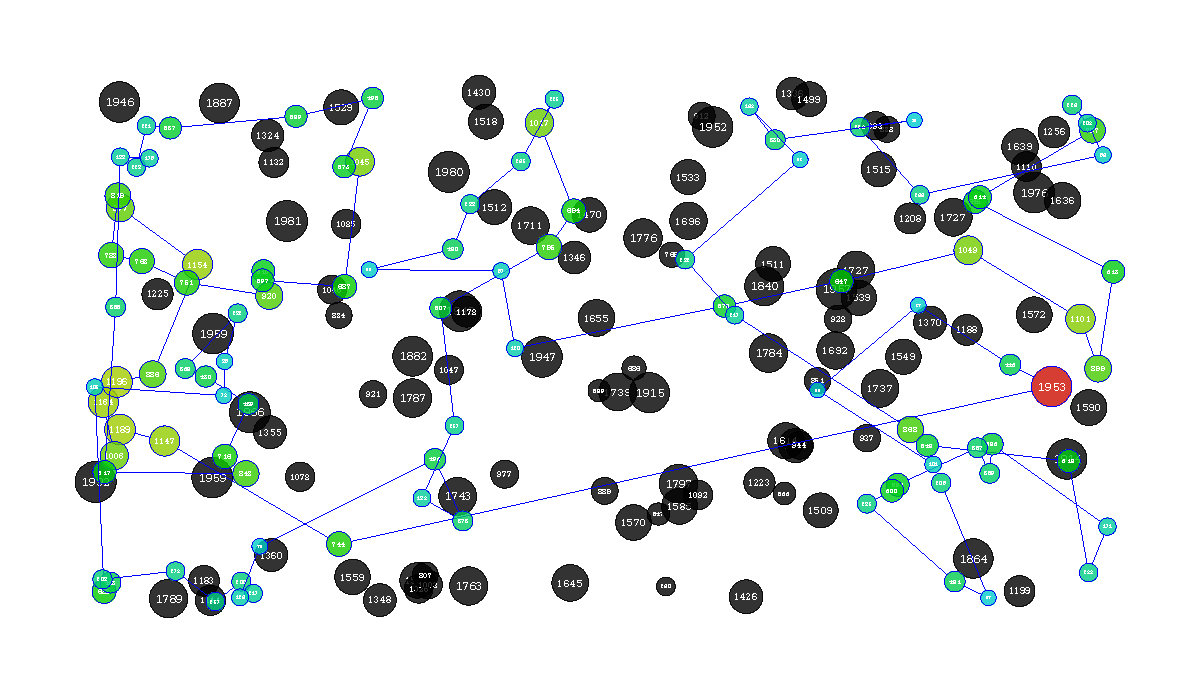
\includegraphics{results/best_nearest-neighbor_TSPB.pdf}
	\end{adjustwidth}
	\vspace{-15mm}
	\caption{Best nearest neighbor solution to TSPB (106,815)}
\end{figure}
\begin{figure}[H]
	\begin{adjustwidth}{-3em}{0}
		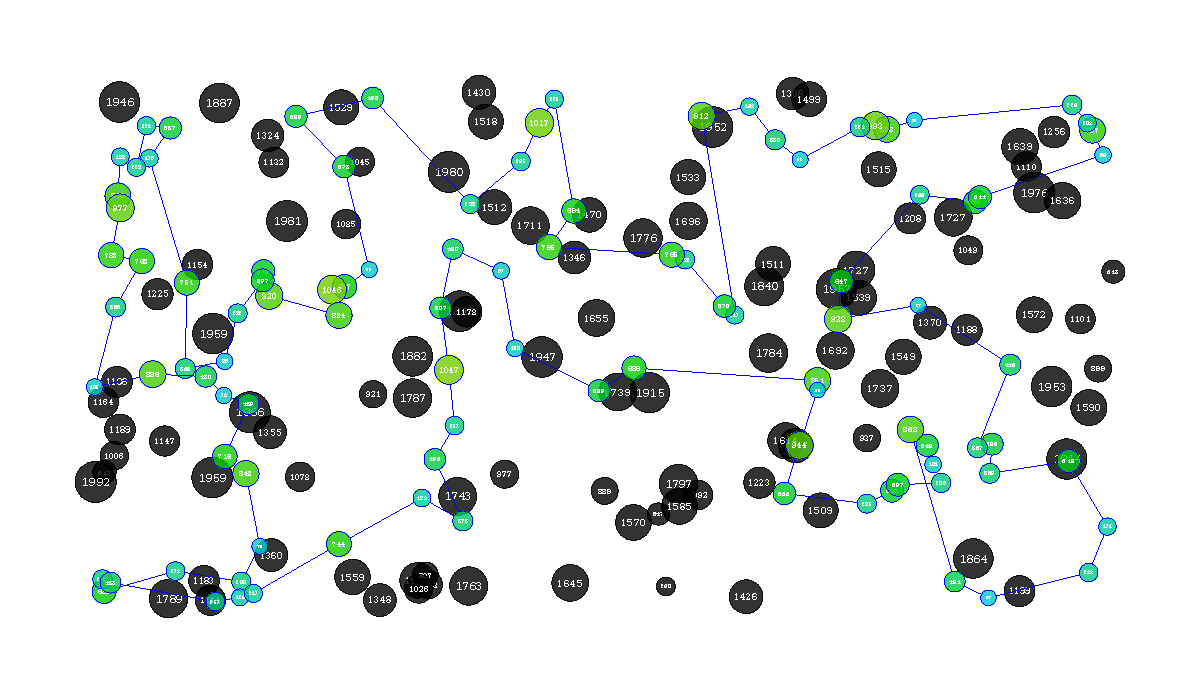
\includegraphics{results/best_greedy-cycle_TSPB.pdf}
	\end{adjustwidth}
	\vspace{-15mm}
	\caption{Best greedy cycle solution to TSPB (111,981)}
\end{figure}

\subsection{TSPC.csv}
\begin{figure}[H]
	\begin{adjustwidth}{-3em}{0}
		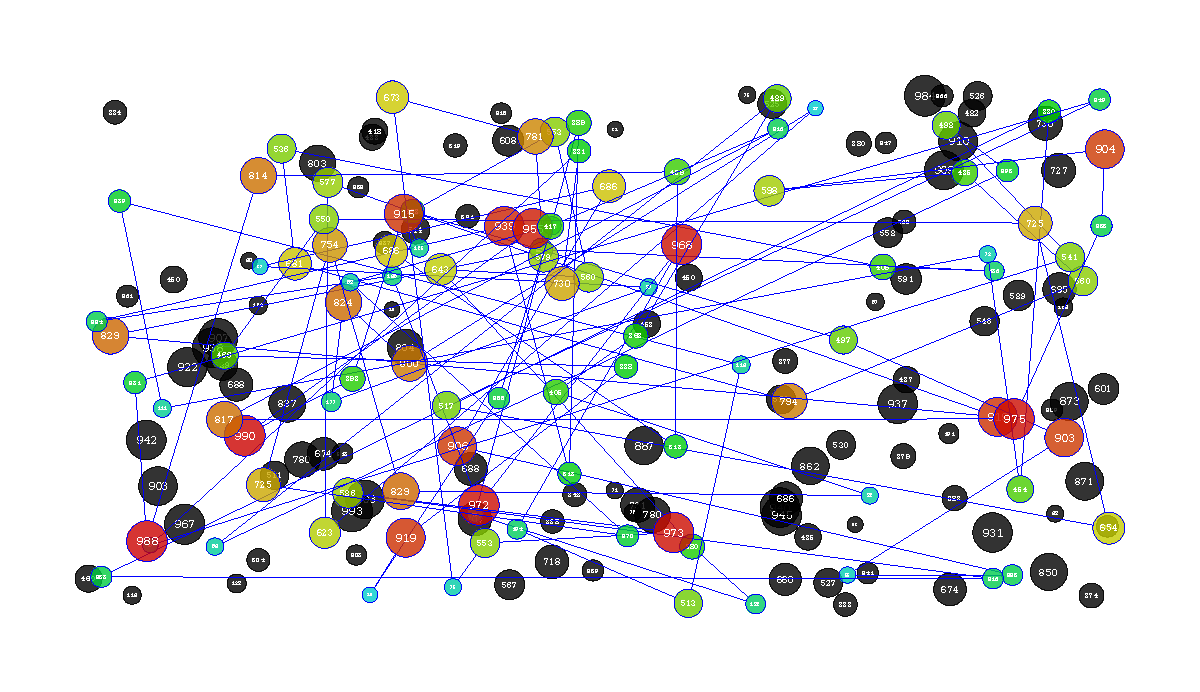
\includegraphics{results/best_random_TSPC.pdf}
	\end{adjustwidth}
	\vspace{-15mm}
	\caption{Best random solution to TSPC (189,473)}
\end{figure}
\begin{figure}[H]
	\begin{adjustwidth}{-3em}{0}
		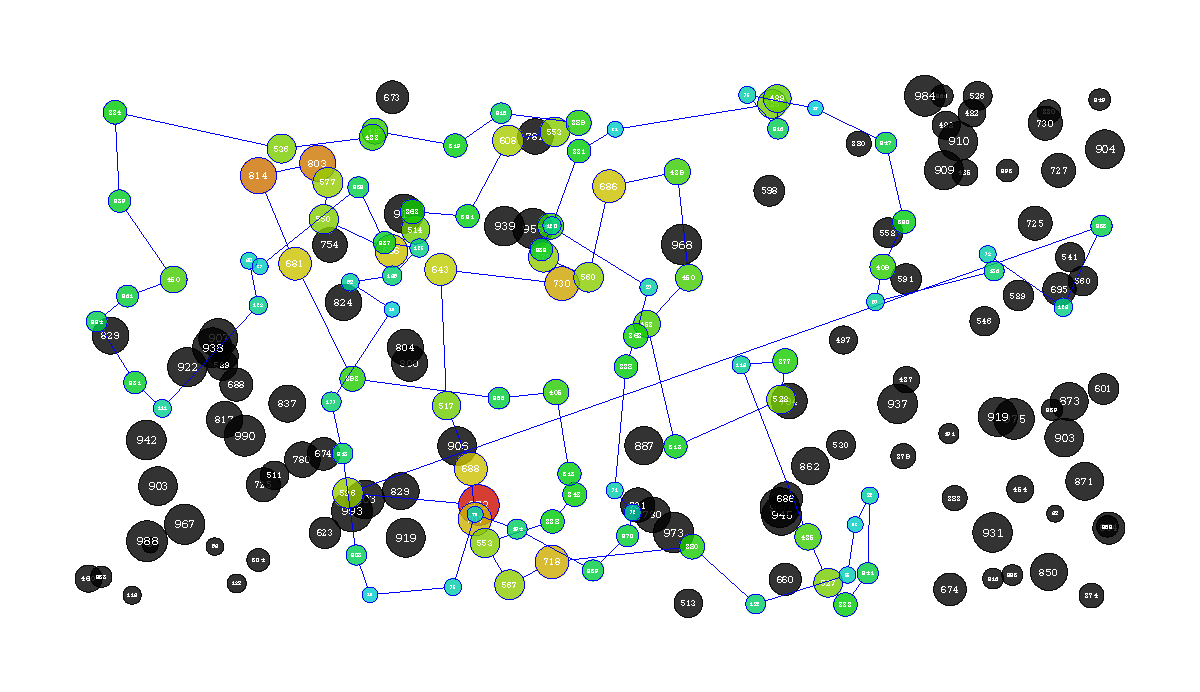
\includegraphics{results/best_nearest-neighbor_TSPC.pdf}
	\end{adjustwidth}
	\vspace{-15mm}
	\caption{Best nearest neighbor solution to TSPC (62,629)}
\end{figure}
\begin{figure}[H]
	\begin{adjustwidth}{-3em}{0}
		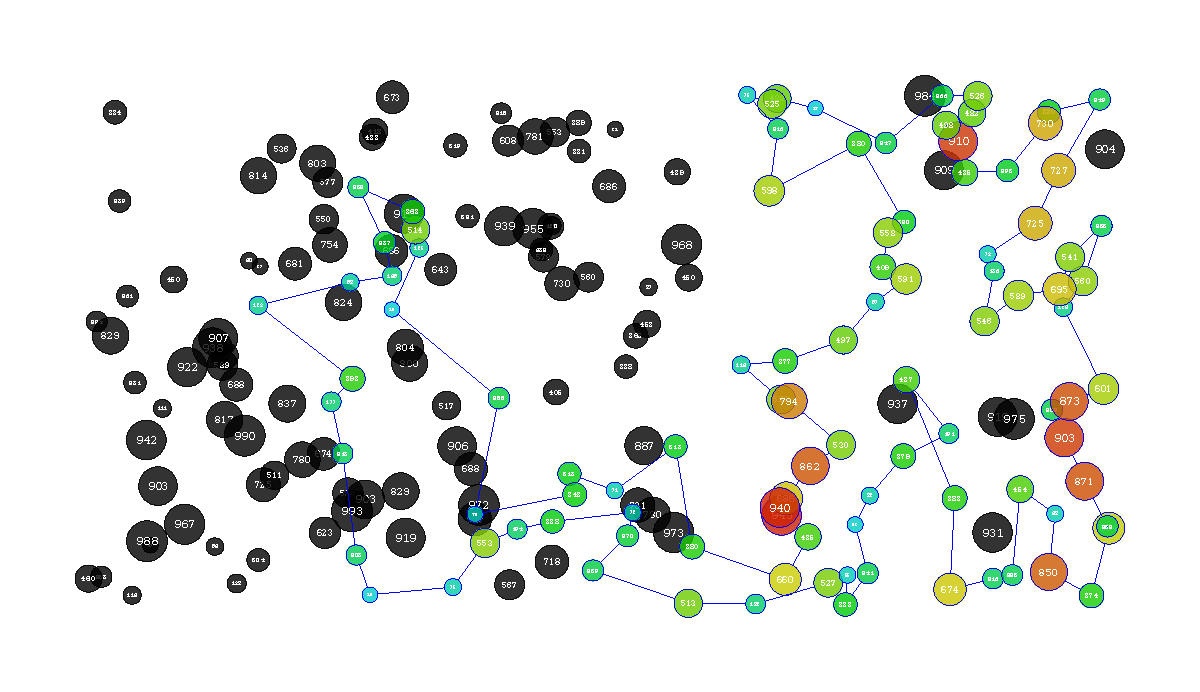
\includegraphics{results/best_greedy-cycle_TSPC.pdf}
	\end{adjustwidth}
	\vspace{-15mm}
	\caption{Best greedy cycle solution to TSPC (67,077)}
\end{figure}

\section{Source code}
The source code for all the experiments and this report is hosted on GitHub: \\
\url{https://github.com/RoyalDonkey/put-ec-tasks}

\section{Conclusions}
The nearest neighbor method actually tends to outperform greedy cycle, despite
the latter being slightly more complex and thus making it seem like it should
be better.

Before I \emph{consciously} read the part of the task description that
specifies to use a cached distance matrix, I was just computing euclidean
distance from scratch each time it was needed. This led to pretty bad
times\footnote{"bad times" = >8 seconds. For comparison, the current and final
version of the program using the distance matrix takes about 5 seconds to run
on my machine.}. I tried a hashmap cache approach, however it actually made
things far worse, because computing euclidean distance is \emph{not} slower
than hashing 2 points, walking through a bucket list and comparing keys. It's
not very common that functions that are already small and quite fast are the
bottleneck, so I was very surprised at this result. Serves as a reminder to
stop and think more often whether a tool is right for the job before we sink
time into it.
\end{document}
